%!TEX root = ../Main.tex

\section{Simulation of Optimal Defense Strategy Generator}

\begin{frame}{Decision-Making Detail 1}
  \begin{overlayarea}{\textwidth}{7cm}
  If the evidence list is $(a_1, a_2)$, the detail of the decision-making is shown as follows.\vspace{5pt}
  \begin{center}
    \scalebox{1}{
    %!TEX root = ../Main.tex

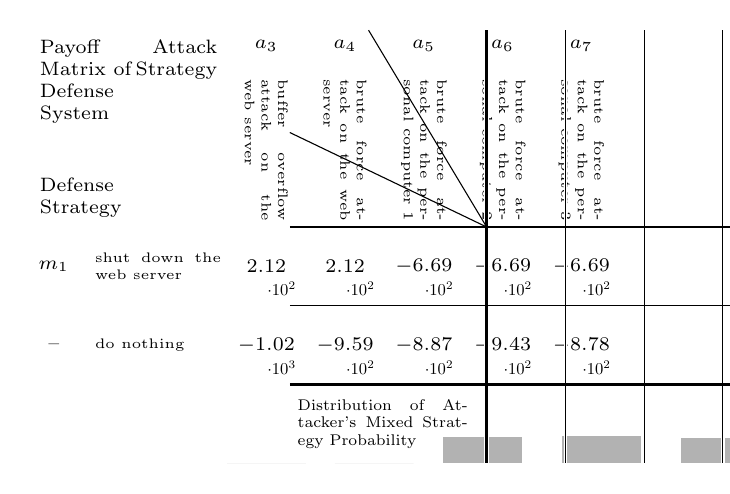
\begin{tikzpicture}
[line width = 0.4pt,
attack/.style = {anchor = north, align =center, font = \scriptsize},
attackdescription/.style = {anchor = west, align = left, font = \tiny, rotate = 270},
defense/.style = {align = center, font = \scriptsize},
defensedescription/.style = {anchor = west, align = left, font = \tiny}]
\linespread{1}
\node[anchor = north east, align = right, font = \scriptsize] at (2.5, 10) {Attack\\Strategy};
\node[anchor = south west, align = left, font = \scriptsize] at (0, 7.5) {Defense\\Strategy};
\node[anchor = north west, align = left, font = \scriptsize] at (0, 10) {Payoff\\Matrix of\\Defense\\System};
\node[defense] at (0.3, 7) {$m_{1}$};
\node[defensedescription] at (0.7, 7) {\parbox{1.6cm}{shut down the web server}};
\node[defense] at (0.3, 6) {--};
\node[defensedescription] at (0.7, 6) {\parbox{1.6cm}{do nothing}};
\node[attack] at (3, 10) {$a_{3}$};
\node[attackdescription] at (3, 9.5) {\parbox{1.8cm}{buffer overflow attack on the web server}};
\node[attack] at (4, 10) {$a_{4}$};
\node[attackdescription] at (4, 9.5) {\parbox{1.8cm}{brute force attack on the web server}};
\node[attack] at (5, 10) {$a_{5}$};
\node[attackdescription] at (5, 9.5) {\parbox{1.8cm}{brute force attack on the personal computer 1}};
\node[attack] at (6, 10) {$a_{6}$};
\node[attackdescription] at (6, 9.5) {\parbox{1.8cm}{brute force attack on the personal computer 2}};
\node[attack] at (7, 10) {$a_{7}$};
\node[attackdescription] at (7, 9.5) {\parbox{1.8cm}{brute force attack on the personal computer 3}};
\node[font = \scriptsize] at (3, 7) {$2.12$};
\node[anchor = south east] at (3.5, 6.5) {\scalebox{0.6}{$\cdot 10^{2}$}};
\node[font = \scriptsize] at (4, 7) {$2.12$};
\node[anchor = south east] at (4.5, 6.5) {\scalebox{0.6}{$\cdot 10^{2}$}};
\node[font = \scriptsize] at (5, 7) {$-6.69$};
\node[anchor = south east] at (5.5, 6.5) {\scalebox{0.6}{$\cdot 10^{2}$}};
\node[font = \scriptsize] at (6, 7) {$-6.69$};
\node[anchor = south east] at (6.5, 6.5) {\scalebox{0.6}{$\cdot 10^{2}$}};
\node[font = \scriptsize] at (7, 7) {$-6.69$};
\node[anchor = south east] at (7.5, 6.5) {\scalebox{0.6}{$\cdot 10^{2}$}};
\node[font = \scriptsize] at (3, 6) {$-1.02$};
\node[anchor = south east] at (3.5, 5.5) {\scalebox{0.6}{$\cdot 10^{3}$}};
\node[font = \scriptsize] at (4, 6) {$-9.59$};
\node[anchor = south east] at (4.5, 5.5) {\scalebox{0.6}{$\cdot 10^{2}$}};
\node[font = \scriptsize] at (5, 6) {$-8.87$};
\node[anchor = south east] at (5.5, 5.5) {\scalebox{0.6}{$\cdot 10^{2}$}};
\node[font = \scriptsize] at (6, 6) {$-9.43$};
\node[anchor = south east] at (6.5, 5.5) {\scalebox{0.6}{$\cdot 10^{2}$}};
\node[font = \scriptsize] at (7, 6) {$-8.78$};
\node[anchor = south east] at (7.5, 5.5) {\scalebox{0.6}{$\cdot 10^{2}$}};
\fill[black!30] (2.5, 4.5) -- (3.5, 4.5) -- (3.5, 4.5) -- (2.5, 4.5) -- cycle;
\shadowtext[font = \scriptsize] at (3, 5) {$0\%$};
\fill[black!30] (3.5, 4.5) -- (4.5, 4.5) -- (4.5, 4.5) -- (3.5, 4.5) -- cycle;
\shadowtext[font = \scriptsize] at (4, 5) {$0\%$};
\fill[black!30] (4.5, 4.5) -- (5.5, 4.5) -- (5.5, 4.8274) -- (4.5, 4.8274) -- cycle;
\shadowtext[font = \scriptsize] at (5, 5) {$33\%$};
\fill[black!30] (5.5, 4.5) -- (6.5, 4.5) -- (6.5, 4.8488) -- (5.5, 4.8488) -- cycle;
\shadowtext[font = \scriptsize] at (6, 5) {$35\%$};
\fill[black!30] (6.5, 4.5) -- (7.5, 4.5) -- (7.5, 4.8238) -- (6.5, 4.8238) -- cycle;
\shadowtext[font = \scriptsize] at (7, 5) {$32\%$};
\fill[black!30] (8.5, 7.5) -- (8.5, 6.5) -- (7.53, 6.5) -- (7.53, 7.5) -- cycle;
\shadowtext[font = \scriptsize] at (8, 7) {$100\%$};
\fill[black!30] (8.5, 6.5) -- (8.5, 5.5) -- (8.5, 5.5) -- (8.5, 6.5) -- cycle;
\shadowtext[font = \scriptsize] at (8, 6) {$0\%$};
\node[anchor = west] at (0, 5) {\scalebox{0.8}{\parbox{2.7cm}{\scriptsize Distribution of Attacker's Mixed Strategy Probability}}};
\node[anchor = west, rotate = -90] at (8, 10) {\scalebox{0.8}{\parbox{2.7cm}{\scriptsize Distribution of defense System's Mixed Strategy Probability}}};
\draw[line width = 1.2pt, white] (0, 6.5) -- (8.5 ,6.5);
\draw[line width = 1.2pt, white] (0, 5.5) -- (8.5 ,5.5);
\draw[line width = 1.8pt, white] (0, 5.5) -- (8.5 ,5.5);
\draw[line width = 1.8pt, white] (0, 7.5) -- (8.5 ,7.5);
\draw[line width = 1.2pt, white] (2.5, 10) -- (2.5, 4.5);
\draw[line width = 1.2pt, white] (3.5, 10) -- (3.5, 4.5);
\draw[line width = 1.2pt, white] (4.5, 10) -- (4.5, 4.5);
\draw[line width = 1.2pt, white] (5.5, 10) -- (5.5, 4.5);
\draw[line width = 1.2pt, white] (6.5, 10) -- (6.5, 4.5);
\draw[line width = 1.8pt, white] (7.5, 10) -- (7.5, 4.5);
\draw[line width = 1.8pt, white] (2.5, 10) -- (2.5,4.5);
\draw (0, 6.5) -- (8.5 ,6.5);
\draw (0, 5.5) -- (8.5 ,5.5);
\draw[line width = 1pt] (0, 5.5) -- (8.5 ,5.5);
\draw[line width = 1pt] (0, 7.5) -- (8.5 ,7.5);
\draw (2.5, 10) -- (2.5, 4.5);
\draw (3.5, 10) -- (3.5, 4.5);
\draw (4.5, 10) -- (4.5, 4.5);
\draw (5.5, 10) -- (5.5, 4.5);
\draw (6.5, 10) -- (6.5, 4.5);
\draw[line width = 1pt] (7.5, 10) -- (7.5, 4.5);
\draw[line width = 1pt] (2.5, 10) -- (2.5,4.5);

\draw (0, 8.7) -- (2.5, 7.5);
\draw (1, 10) -- (2.5, 7.5);
\end{tikzpicture}
    }
  \end{center}
  \end{overlayarea}
\end{frame}

\begin{frame}{Decision-Making Detail 2}
  \begin{overlayarea}{\textwidth}{7cm}
  If the evidence list is $(a_1, a_2, a_3, a_8, a_9, a_{10}, a_{25}, f_8)$, the detail of the decision-making is shown as follows.
  \begin{center}
    \scalebox{0.7}{
    %!TEX root = ../Main.tex

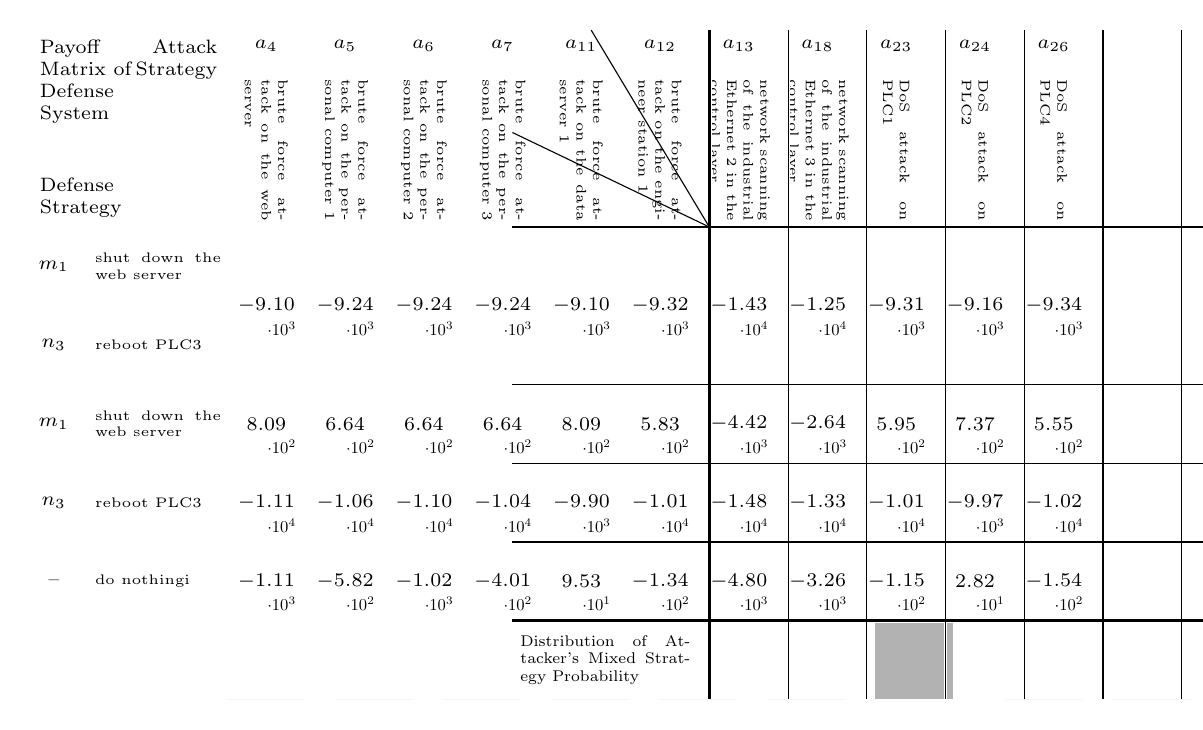
\begin{tikzpicture}
[line width = 0.4pt,
attack/.style = {anchor = north, align =center, font = \scriptsize},
attackdescription/.style = {anchor = west, align = left, font = \tiny, rotate = 270, text = black},
defense/.style = {align = center, font = \scriptsize},
defensedescription/.style = {anchor = west, align = left, font = \tiny}]
\linespread{1}
\node[anchor = north east, align = right, font = \scriptsize] at (2.5, 10) {Attack\\Strategy};
\node[anchor = south west, align = left, font = \scriptsize] at (0, 7.5) {Defense\\Strategy};
\node[anchor = north west, align = left, font = \scriptsize] at (0, 10) {Payoff\\Matrix of\\Defense\\System};
\node[defense] at (0.3, 7) {$m_{1}$};
\node[defensedescription] at (0.7, 7) {\parbox{1.6cm}{shut down the web server}};
\node[defense] at (0.3, 6) {$n_{3}$};
\node[defensedescription] at (0.7, 6) {\parbox{1.6cm}{reboot PLC3}};
\node[defense] at (0.3, 5) {$m_{1}$};
\node[defensedescription] at (0.7, 5) {\parbox{1.6cm}{shut down the web server}};
\node[defense] at (0.3, 4) {$n_{3}$};
\node[defensedescription] at (0.7, 4) {\parbox{1.6cm}{reboot PLC3}};
\node[defense] at (0.3, 3) {--};
\node[defensedescription] at (0.7, 3) {\parbox{1.6cm}{do nothingi}};
\node[attack] at (3, 10) {$a_{4}$};
\node[attackdescription] at (3, 9.5) {\parbox{1.8cm}{brute force attack on the web server}};
\node[attack] at (4, 10) {$a_{5}$};
\node[attackdescription] at (4, 9.5) {\parbox{1.8cm}{brute force attack on the personal computer 1}};
\node[attack] at (5, 10) {$a_{6}$};
\node[attackdescription] at (5, 9.5) {\parbox{1.8cm}{brute force attack on the personal computer 2}};
\node[attack] at (6, 10) {$a_{7}$};
\node[attackdescription] at (6, 9.5) {\parbox{1.8cm}{brute force attack on the personal computer 3}};
\node[attack] at (7, 10) {$a_{11}$};
\node[attackdescription] at (7, 9.5) {\parbox{1.8cm}{brute force attack on the data server 1}};
\node[attack] at (8, 10) {$a_{12}$};
\node[attackdescription] at (8, 9.5) {\parbox{1.8cm}{brute force attack on the engineer station 1}};
\node[attack] at (9, 10) {$a_{13}$};
\node[attackdescription] at (9, 9.5) {\parbox{1.8cm}{network scanning of the industrial Ethernet 2 in the control layer}};
\node[attack] at (10, 10) {$a_{18}$};
\node[attackdescription] at (10, 9.5) {\parbox{1.8cm}{network scanning of the industrial Ethernet 3 in the control layer}};
\node[attack] at (11, 10) {$a_{23}$};
\node[attackdescription] at (11, 9.5) {\parbox{1.8cm}{DoS attack on PLC1}};
\node[attack] at (12, 10) {$a_{24}$};
\node[attackdescription] at (12, 9.5) {\parbox{1.8cm}{DoS attack on PLC2}};
\node[attack] at (13, 10) {$a_{26}$};
\node[attackdescription] at (13, 9.5) {\parbox{1.8cm}{DoS attack on PLC4}};
\node[font = \scriptsize] at (3, 6.5) {$-9.10$};
\node[anchor = south east] at (3.5, 6) {\scalebox{0.6}{$\cdot 10^{3}$}};
\node[font = \scriptsize] at (4, 6.5) {$-9.24$};
\node[anchor = south east] at (4.5, 6) {\scalebox{0.6}{$\cdot 10^{3}$}};
\node[font = \scriptsize] at (5, 6.5) {$-9.24$};
\node[anchor = south east] at (5.5, 6) {\scalebox{0.6}{$\cdot 10^{3}$}};
\node[font = \scriptsize] at (6, 6.5) {$-9.24$};
\node[anchor = south east] at (6.5, 6) {\scalebox{0.6}{$\cdot 10^{3}$}};
\node[font = \scriptsize] at (7, 6.5) {$-9.10$};
\node[anchor = south east] at (7.5, 6) {\scalebox{0.6}{$\cdot 10^{3}$}};
\node[font = \scriptsize] at (8, 6.5) {$-9.32$};
\node[anchor = south east] at (8.5, 6) {\scalebox{0.6}{$\cdot 10^{3}$}};
\node[font = \scriptsize] at (9, 6.5) {$-1.43$};
\node[anchor = south east] at (9.5, 6) {\scalebox{0.6}{$\cdot 10^{4}$}};
\node[font = \scriptsize] at (10, 6.5) {$-1.25$};
\node[anchor = south east] at (10.5, 6) {\scalebox{0.6}{$\cdot 10^{4}$}};
\node[font = \scriptsize] at (11, 6.5) {$-9.31$};
\node[anchor = south east] at (11.5, 6) {\scalebox{0.6}{$\cdot 10^{3}$}};
\node[font = \scriptsize] at (12, 6.5) {$-9.16$};
\node[anchor = south east] at (12.5, 6) {\scalebox{0.6}{$\cdot 10^{3}$}};
\node[font = \scriptsize] at (13, 6.5) {$-9.34$};
\node[anchor = south east] at (13.5, 6) {\scalebox{0.6}{$\cdot 10^{3}$}};
\node[font = \scriptsize] at (3, 5) {$8.09$};
\node[anchor = south east] at (3.5, 4.5) {\scalebox{0.6}{$\cdot 10^{2}$}};
\node[font = \scriptsize] at (4, 5) {$6.64$};
\node[anchor = south east] at (4.5, 4.5) {\scalebox{0.6}{$\cdot 10^{2}$}};
\node[font = \scriptsize] at (5, 5) {$6.64$};
\node[anchor = south east] at (5.5, 4.5) {\scalebox{0.6}{$\cdot 10^{2}$}};
\node[font = \scriptsize] at (6, 5) {$6.64$};
\node[anchor = south east] at (6.5, 4.5) {\scalebox{0.6}{$\cdot 10^{2}$}};
\node[font = \scriptsize] at (7, 5) {$8.09$};
\node[anchor = south east] at (7.5, 4.5) {\scalebox{0.6}{$\cdot 10^{2}$}};
\node[font = \scriptsize] at (8, 5) {$5.83$};
\node[anchor = south east] at (8.5, 4.5) {\scalebox{0.6}{$\cdot 10^{2}$}};
\node[font = \scriptsize] at (9, 5) {$-4.42$};
\node[anchor = south east] at (9.5, 4.5) {\scalebox{0.6}{$\cdot 10^{3}$}};
\node[font = \scriptsize] at (10, 5) {$-2.64$};
\node[anchor = south east] at (10.5, 4.5) {\scalebox{0.6}{$\cdot 10^{3}$}};
\node[font = \scriptsize] at (11, 5) {$5.95$};
\node[anchor = south east] at (11.5, 4.5) {\scalebox{0.6}{$\cdot 10^{2}$}};
\node[font = \scriptsize] at (12, 5) {$7.37$};
\node[anchor = south east] at (12.5, 4.5) {\scalebox{0.6}{$\cdot 10^{2}$}};
\node[font = \scriptsize] at (13, 5) {$5.55$};
\node[anchor = south east] at (13.5, 4.5) {\scalebox{0.6}{$\cdot 10^{2}$}};
\node[font = \scriptsize] at (3, 4) {$-1.11$};
\node[anchor = south east] at (3.5, 3.5) {\scalebox{0.6}{$\cdot 10^{4}$}};
\node[font = \scriptsize] at (4, 4) {$-1.06$};
\node[anchor = south east] at (4.5, 3.5) {\scalebox{0.6}{$\cdot 10^{4}$}};
\node[font = \scriptsize] at (5, 4) {$-1.10$};
\node[anchor = south east] at (5.5, 3.5) {\scalebox{0.6}{$\cdot 10^{4}$}};
\node[font = \scriptsize] at (6, 4) {$-1.04$};
\node[anchor = south east] at (6.5, 3.5) {\scalebox{0.6}{$\cdot 10^{4}$}};
\node[font = \scriptsize] at (7, 4) {$-9.90$};
\node[anchor = south east] at (7.5, 3.5) {\scalebox{0.6}{$\cdot 10^{3}$}};
\node[font = \scriptsize] at (8, 4) {$-1.01$};
\node[anchor = south east] at (8.5, 3.5) {\scalebox{0.6}{$\cdot 10^{4}$}};
\node[font = \scriptsize] at (9, 4) {$-1.48$};
\node[anchor = south east] at (9.5, 3.5) {\scalebox{0.6}{$\cdot 10^{4}$}};
\node[font = \scriptsize] at (10, 4) {$-1.33$};
\node[anchor = south east] at (10.5, 3.5) {\scalebox{0.6}{$\cdot 10^{4}$}};
\node[font = \scriptsize] at (11, 4) {$-1.01$};
\node[anchor = south east] at (11.5, 3.5) {\scalebox{0.6}{$\cdot 10^{4}$}};
\node[font = \scriptsize] at (12, 4) {$-9.97$};
\node[anchor = south east] at (12.5, 3.5) {\scalebox{0.6}{$\cdot 10^{3}$}};
\node[font = \scriptsize] at (13, 4) {$-1.02$};
\node[anchor = south east] at (13.5, 3.5) {\scalebox{0.6}{$\cdot 10^{4}$}};
\node[font = \scriptsize] at (3, 3) {$-1.11$};
\node[anchor = south east] at (3.5, 2.5) {\scalebox{0.6}{$\cdot 10^{3}$}};
\node[font = \scriptsize] at (4, 3) {$-5.82$};
\node[anchor = south east] at (4.5, 2.5) {\scalebox{0.6}{$\cdot 10^{2}$}};
\node[font = \scriptsize] at (5, 3) {$-1.02$};
\node[anchor = south east] at (5.5, 2.5) {\scalebox{0.6}{$\cdot 10^{3}$}};
\node[font = \scriptsize] at (6, 3) {$-4.01$};
\node[anchor = south east] at (6.5, 2.5) {\scalebox{0.6}{$\cdot 10^{2}$}};
\node[font = \scriptsize] at (7, 3) {$9.53$};
\node[anchor = south east] at (7.5, 2.5) {\scalebox{0.6}{$\cdot 10^{1}$}};
\node[font = \scriptsize] at (8, 3) {$-1.34$};
\node[anchor = south east] at (8.5, 2.5) {\scalebox{0.6}{$\cdot 10^{2}$}};
\node[font = \scriptsize] at (9, 3) {$-4.80$};
\node[anchor = south east] at (9.5, 2.5) {\scalebox{0.6}{$\cdot 10^{3}$}};
\node[font = \scriptsize] at (10, 3) {$-3.26$};
\node[anchor = south east] at (10.5, 2.5) {\scalebox{0.6}{$\cdot 10^{3}$}};
\node[font = \scriptsize] at (11, 3) {$-1.15$};
\node[anchor = south east] at (11.5, 2.5) {\scalebox{0.6}{$\cdot 10^{2}$}};
\node[font = \scriptsize] at (12, 3) {$2.82$};
\node[anchor = south east] at (12.5, 2.5) {\scalebox{0.6}{$\cdot 10^{1}$}};
\node[font = \scriptsize] at (13, 3) {$-1.54$};
\node[anchor = south east] at (13.5, 2.5) {\scalebox{0.6}{$\cdot 10^{2}$}};
\fill[black!30] (2.5, 1.5) -- (3.5, 1.5) -- (3.5, 1.5) -- (2.5, 1.5) -- cycle;
\shadowtext[font = \scriptsize] at (3, 2) {$0\%$};
\fill[black!30] (3.5, 1.5) -- (4.5, 1.5) -- (4.5, 1.5) -- (3.5, 1.5) -- cycle;
\shadowtext[font = \scriptsize] at (4, 2) {$0\%$};
\fill[black!30] (4.5, 1.5) -- (5.5, 1.5) -- (5.5, 1.5) -- (4.5, 1.5) -- cycle;
\shadowtext[font = \scriptsize] at (5, 2) {$0\%$};
\fill[black!30] (5.5, 1.5) -- (6.5, 1.5) -- (6.5, 1.5) -- (5.5, 1.5) -- cycle;
\shadowtext[font = \scriptsize] at (6, 2) {$0\%$};
\fill[black!30] (6.5, 1.5) -- (7.5, 1.5) -- (7.5, 1.5) -- (6.5, 1.5) -- cycle;
\shadowtext[font = \scriptsize] at (7, 2) {$0\%$};
\fill[black!30] (7.5, 1.5) -- (8.5, 1.5) -- (8.5, 1.5) -- (7.5, 1.5) -- cycle;
\shadowtext[font = \scriptsize] at (8, 2) {$0\%$};
\fill[black!30] (8.5, 1.5) -- (9.5, 1.5) -- (9.5, 2.5) -- (8.5, 2.5) -- cycle;
\shadowtext[font = \scriptsize] at (9, 2) {$100\%$};
\fill[black!30] (9.5, 1.5) -- (10.5, 1.5) -- (10.5, 1.5) -- (9.5, 1.5) -- cycle;
\shadowtext[font = \scriptsize] at (10, 2) {$0\%$};
\fill[black!30] (10.5, 1.5) -- (11.5, 1.5) -- (11.5, 1.5) -- (10.5, 1.5) -- cycle;
\shadowtext[font = \scriptsize] at (11, 2) {$0\%$};
\fill[black!30] (11.5, 1.5) -- (12.5, 1.5) -- (12.5, 1.5) -- (11.5, 1.5) -- cycle;
\shadowtext[font = \scriptsize] at (12, 2) {$0\%$};
\fill[black!30] (12.5, 1.5) -- (13.5, 1.5) -- (13.5, 1.5) -- (12.5, 1.5) -- cycle;
\shadowtext[font = \scriptsize] at (13, 2) {$0\%$};
\fill[black!30] (14.5, 7.5) -- (14.5, 5.5) -- (14.5, 5.5) -- (14.5, 7.5) -- cycle;
\shadowtext[font = \scriptsize] at (14, 6.5) {$0\%$};
\fill[black!30] (14.5, 5.5) -- (14.5, 4.5) -- (13.53, 4.5) -- (13.53, 5.5) -- cycle;
\shadowtext[font = \scriptsize] at (14, 5) {$100\%$};
\fill[black!30] (14.5, 4.5) -- (14.5, 3.5) -- (14.5, 3.5) -- (14.5, 4.5) -- cycle;
\shadowtext[font = \scriptsize] at (14, 4) {$0\%$};
\fill[black!30] (14.5, 3.5) -- (14.5, 2.5) -- (14.5, 2.5) -- (14.5, 3.5) -- cycle;
\shadowtext[font = \scriptsize] at (14, 3) {$0\%$};
\node[anchor = west] at (0, 2) {\scalebox{0.8}{\parbox{2.7cm}{\scriptsize Distribution of Attacker's Mixed Strategy Probability}}};
\node[anchor = west, rotate = -90] at (14, 10) {\scalebox{0.8}{\parbox{2.7cm}{\scriptsize Distribution of defense System's Mixed Strategy Probability}}};
\draw[line width = 1.2pt, white] (0, 5.5) -- (14.5 ,5.5);
\draw[line width = 1.2pt, white] (0, 4.5) -- (14.5 ,4.5);
\draw[line width = 1.2pt, white] (0, 3.5) -- (14.5 ,3.5);
\draw[line width = 1.2pt, white] (0, 2.5) -- (14.5 ,2.5);
\draw[line width = 1.8pt, white] (0, 2.5) -- (14.5 ,2.5);
\draw[line width = 1.8pt, white] (0, 7.5) -- (14.5 ,7.5);
\draw[line width = 1.2pt, white] (2.5, 10) -- (2.5, 1.5);
\draw[line width = 1.2pt, white] (3.5, 10) -- (3.5, 1.5);
\draw[line width = 1.2pt, white] (4.5, 10) -- (4.5, 1.5);
\draw[line width = 1.2pt, white] (5.5, 10) -- (5.5, 1.5);
\draw[line width = 1.2pt, white] (6.5, 10) -- (6.5, 1.5);
\draw[line width = 1.2pt, white] (7.5, 10) -- (7.5, 1.5);
\draw[line width = 1.2pt, white] (8.5, 10) -- (8.5, 1.5);
\draw[line width = 1.2pt, white] (9.5, 10) -- (9.5, 1.5);
\draw[line width = 1.2pt, white] (10.5, 10) -- (10.5, 1.5);
\draw[line width = 1.2pt, white] (11.5, 10) -- (11.5, 1.5);
\draw[line width = 1.2pt, white] (12.5, 10) -- (12.5, 1.5);
\draw[line width = 1.8pt, white] (13.5, 10) -- (13.5, 1.5);
\draw[line width = 1.8pt, white] (2.5, 10) -- (2.5,1.5);
\draw (0, 5.5) -- (14.5 ,5.5);
\draw (0, 4.5) -- (14.5 ,4.5);
\draw (0, 3.5) -- (14.5 ,3.5);
\draw (0, 2.5) -- (14.5 ,2.5);
\draw[line width = 1pt] (0, 2.5) -- (14.5 ,2.5);
\draw[line width = 1pt] (0, 7.5) -- (14.5 ,7.5);
\draw (2.5, 10) -- (2.5, 1.5);
\draw (3.5, 10) -- (3.5, 1.5);
\draw (4.5, 10) -- (4.5, 1.5);
\draw (5.5, 10) -- (5.5, 1.5);
\draw (6.5, 10) -- (6.5, 1.5);
\draw (7.5, 10) -- (7.5, 1.5);
\draw (8.5, 10) -- (8.5, 1.5);
\draw (9.5, 10) -- (9.5, 1.5);
\draw (10.5, 10) -- (10.5, 1.5);
\draw (11.5, 10) -- (11.5, 1.5);
\draw (12.5, 10) -- (12.5, 1.5);
\draw[line width = 1pt] (13.5, 10) -- (13.5, 1.5);
\draw[line width = 1pt] (2.5, 10) -- (2.5,1.5);

\draw (0, 8.7) -- (2.5, 7.5);
\draw (1, 10) -- (2.5, 7.5);
\end{tikzpicture}
    }
  \end{center}
  \end{overlayarea}
\end{frame}

\begin{frame}{Decision-Making Detail 3}
  \begin{overlayarea}{\textwidth}{7cm}
  New, the cost of recovery strategy $n_3$ is reduced to $0$, the detail of the decision-making is shown as follows.
  \begin{center}
    \scalebox{0.7}{
    %!TEX root = ../Main.tex

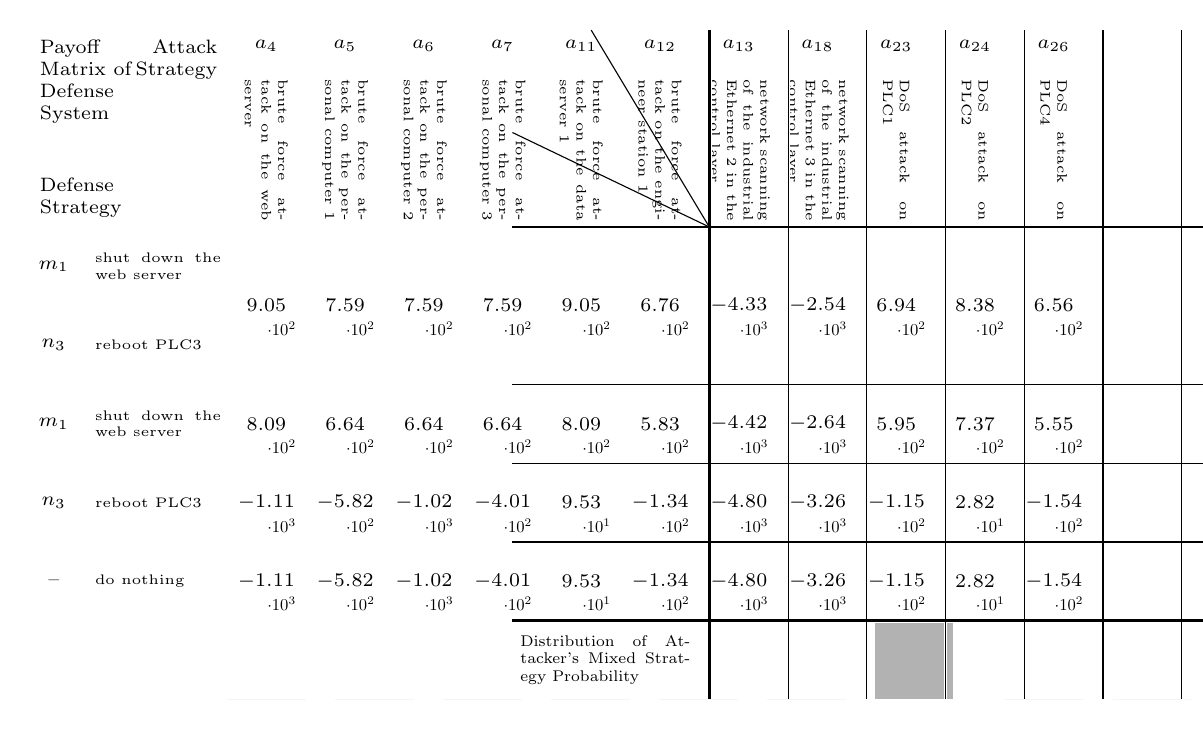
\begin{tikzpicture}
[line width = 0.4pt,
attack/.style = {anchor = north, align =center, font = \scriptsize},
attackdescription/.style = {anchor = west, align = left, font = \tiny, rotate = 270},
defense/.style = {align = center, font = \scriptsize},
defensedescription/.style = {anchor = west, align = left, font = \tiny}]
\linespread{1}
\node[anchor = north east, align = right, font = \scriptsize] at (2.5, 10) {Attack\\Strategy};
\node[anchor = south west, align = left, font = \scriptsize] at (0, 7.5) {Defense\\Strategy};
\node[anchor = north west, align = left, font = \scriptsize] at (0, 10) {Payoff\\Matrix of\\Defense\\System};
\node[defense] at (0.3, 7) {$m_{1}$};
\node[defensedescription] at (0.7, 7) {\parbox{1.6cm}{shut down the web server}};
\node[defense] at (0.3, 6) {$n_{3}$};
\node[defensedescription] at (0.7, 6) {\parbox{1.6cm}{reboot PLC3}};
\node[defense] at (0.3, 5) {$m_{1}$};
\node[defensedescription] at (0.7, 5) {\parbox{1.6cm}{shut down the web server}};
\node[defense] at (0.3, 4) {$n_{3}$};
\node[defensedescription] at (0.7, 4) {\parbox{1.6cm}{reboot PLC3}};
\node[defense] at (0.3, 3) {--};
\node[defensedescription] at (0.7, 3) {\parbox{1.6cm}{do nothing}};
\node[attack] at (3, 10) {$a_{4}$};
\node[attackdescription] at (3, 9.5) {\parbox{1.8cm}{brute force attack on the web server}};
\node[attack] at (4, 10) {$a_{5}$};
\node[attackdescription] at (4, 9.5) {\parbox{1.8cm}{brute force attack on the personal computer 1}};
\node[attack] at (5, 10) {$a_{6}$};
\node[attackdescription] at (5, 9.5) {\parbox{1.8cm}{brute force attack on the personal computer 2}};
\node[attack] at (6, 10) {$a_{7}$};
\node[attackdescription] at (6, 9.5) {\parbox{1.8cm}{brute force attack on the personal computer 3}};
\node[attack] at (7, 10) {$a_{11}$};
\node[attackdescription] at (7, 9.5) {\parbox{1.8cm}{brute force attack on the data server 1}};
\node[attack] at (8, 10) {$a_{12}$};
\node[attackdescription] at (8, 9.5) {\parbox{1.8cm}{brute force attack on the engineer station 1}};
\node[attack] at (9, 10) {$a_{13}$};
\node[attackdescription] at (9, 9.5) {\parbox{1.8cm}{network scanning of the industrial Ethernet 2 in the control layer}};
\node[attack] at (10, 10) {$a_{18}$};
\node[attackdescription] at (10, 9.5) {\parbox{1.8cm}{network scanning of the industrial Ethernet 3 in the control layer}};
\node[attack] at (11, 10) {$a_{23}$};
\node[attackdescription] at (11, 9.5) {\parbox{1.8cm}{DoS attack on PLC1}};
\node[attack] at (12, 10) {$a_{24}$};
\node[attackdescription] at (12, 9.5) {\parbox{1.8cm}{DoS attack on PLC2}};
\node[attack] at (13, 10) {$a_{26}$};
\node[attackdescription] at (13, 9.5) {\parbox{1.8cm}{DoS attack on PLC4}};
\node[font = \scriptsize] at (3, 6.5) {$9.05$};
\node[anchor = south east] at (3.5, 6) {\scalebox{0.6}{$\cdot 10^{2}$}};
\node[font = \scriptsize] at (4, 6.5) {$7.59$};
\node[anchor = south east] at (4.5, 6) {\scalebox{0.6}{$\cdot 10^{2}$}};
\node[font = \scriptsize] at (5, 6.5) {$7.59$};
\node[anchor = south east] at (5.5, 6) {\scalebox{0.6}{$\cdot 10^{2}$}};
\node[font = \scriptsize] at (6, 6.5) {$7.59$};
\node[anchor = south east] at (6.5, 6) {\scalebox{0.6}{$\cdot 10^{2}$}};
\node[font = \scriptsize] at (7, 6.5) {$9.05$};
\node[anchor = south east] at (7.5, 6) {\scalebox{0.6}{$\cdot 10^{2}$}};
\node[font = \scriptsize] at (8, 6.5) {$6.76$};
\node[anchor = south east] at (8.5, 6) {\scalebox{0.6}{$\cdot 10^{2}$}};
\node[font = \scriptsize] at (9, 6.5) {$-4.33$};
\node[anchor = south east] at (9.5, 6) {\scalebox{0.6}{$\cdot 10^{3}$}};
\node[font = \scriptsize] at (10, 6.5) {$-2.54$};
\node[anchor = south east] at (10.5, 6) {\scalebox{0.6}{$\cdot 10^{3}$}};
\node[font = \scriptsize] at (11, 6.5) {$6.94$};
\node[anchor = south east] at (11.5, 6) {\scalebox{0.6}{$\cdot 10^{2}$}};
\node[font = \scriptsize] at (12, 6.5) {$8.38$};
\node[anchor = south east] at (12.5, 6) {\scalebox{0.6}{$\cdot 10^{2}$}};
\node[font = \scriptsize] at (13, 6.5) {$6.56$};
\node[anchor = south east] at (13.5, 6) {\scalebox{0.6}{$\cdot 10^{2}$}};
\node[font = \scriptsize] at (3, 5) {$8.09$};
\node[anchor = south east] at (3.5, 4.5) {\scalebox{0.6}{$\cdot 10^{2}$}};
\node[font = \scriptsize] at (4, 5) {$6.64$};
\node[anchor = south east] at (4.5, 4.5) {\scalebox{0.6}{$\cdot 10^{2}$}};
\node[font = \scriptsize] at (5, 5) {$6.64$};
\node[anchor = south east] at (5.5, 4.5) {\scalebox{0.6}{$\cdot 10^{2}$}};
\node[font = \scriptsize] at (6, 5) {$6.64$};
\node[anchor = south east] at (6.5, 4.5) {\scalebox{0.6}{$\cdot 10^{2}$}};
\node[font = \scriptsize] at (7, 5) {$8.09$};
\node[anchor = south east] at (7.5, 4.5) {\scalebox{0.6}{$\cdot 10^{2}$}};
\node[font = \scriptsize] at (8, 5) {$5.83$};
\node[anchor = south east] at (8.5, 4.5) {\scalebox{0.6}{$\cdot 10^{2}$}};
\node[font = \scriptsize] at (9, 5) {$-4.42$};
\node[anchor = south east] at (9.5, 4.5) {\scalebox{0.6}{$\cdot 10^{3}$}};
\node[font = \scriptsize] at (10, 5) {$-2.64$};
\node[anchor = south east] at (10.5, 4.5) {\scalebox{0.6}{$\cdot 10^{3}$}};
\node[font = \scriptsize] at (11, 5) {$5.95$};
\node[anchor = south east] at (11.5, 4.5) {\scalebox{0.6}{$\cdot 10^{2}$}};
\node[font = \scriptsize] at (12, 5) {$7.37$};
\node[anchor = south east] at (12.5, 4.5) {\scalebox{0.6}{$\cdot 10^{2}$}};
\node[font = \scriptsize] at (13, 5) {$5.55$};
\node[anchor = south east] at (13.5, 4.5) {\scalebox{0.6}{$\cdot 10^{2}$}};
\node[font = \scriptsize] at (3, 4) {$-1.11$};
\node[anchor = south east] at (3.5, 3.5) {\scalebox{0.6}{$\cdot 10^{3}$}};
\node[font = \scriptsize] at (4, 4) {$-5.82$};
\node[anchor = south east] at (4.5, 3.5) {\scalebox{0.6}{$\cdot 10^{2}$}};
\node[font = \scriptsize] at (5, 4) {$-1.02$};
\node[anchor = south east] at (5.5, 3.5) {\scalebox{0.6}{$\cdot 10^{3}$}};
\node[font = \scriptsize] at (6, 4) {$-4.01$};
\node[anchor = south east] at (6.5, 3.5) {\scalebox{0.6}{$\cdot 10^{2}$}};
\node[font = \scriptsize] at (7, 4) {$9.53$};
\node[anchor = south east] at (7.5, 3.5) {\scalebox{0.6}{$\cdot 10^{1}$}};
\node[font = \scriptsize] at (8, 4) {$-1.34$};
\node[anchor = south east] at (8.5, 3.5) {\scalebox{0.6}{$\cdot 10^{2}$}};
\node[font = \scriptsize] at (9, 4) {$-4.80$};
\node[anchor = south east] at (9.5, 3.5) {\scalebox{0.6}{$\cdot 10^{3}$}};
\node[font = \scriptsize] at (10, 4) {$-3.26$};
\node[anchor = south east] at (10.5, 3.5) {\scalebox{0.6}{$\cdot 10^{3}$}};
\node[font = \scriptsize] at (11, 4) {$-1.15$};
\node[anchor = south east] at (11.5, 3.5) {\scalebox{0.6}{$\cdot 10^{2}$}};
\node[font = \scriptsize] at (12, 4) {$2.82$};
\node[anchor = south east] at (12.5, 3.5) {\scalebox{0.6}{$\cdot 10^{1}$}};
\node[font = \scriptsize] at (13, 4) {$-1.54$};
\node[anchor = south east] at (13.5, 3.5) {\scalebox{0.6}{$\cdot 10^{2}$}};
\node[font = \scriptsize] at (3, 3) {$-1.11$};
\node[anchor = south east] at (3.5, 2.5) {\scalebox{0.6}{$\cdot 10^{3}$}};
\node[font = \scriptsize] at (4, 3) {$-5.82$};
\node[anchor = south east] at (4.5, 2.5) {\scalebox{0.6}{$\cdot 10^{2}$}};
\node[font = \scriptsize] at (5, 3) {$-1.02$};
\node[anchor = south east] at (5.5, 2.5) {\scalebox{0.6}{$\cdot 10^{3}$}};
\node[font = \scriptsize] at (6, 3) {$-4.01$};
\node[anchor = south east] at (6.5, 2.5) {\scalebox{0.6}{$\cdot 10^{2}$}};
\node[font = \scriptsize] at (7, 3) {$9.53$};
\node[anchor = south east] at (7.5, 2.5) {\scalebox{0.6}{$\cdot 10^{1}$}};
\node[font = \scriptsize] at (8, 3) {$-1.34$};
\node[anchor = south east] at (8.5, 2.5) {\scalebox{0.6}{$\cdot 10^{2}$}};
\node[font = \scriptsize] at (9, 3) {$-4.80$};
\node[anchor = south east] at (9.5, 2.5) {\scalebox{0.6}{$\cdot 10^{3}$}};
\node[font = \scriptsize] at (10, 3) {$-3.26$};
\node[anchor = south east] at (10.5, 2.5) {\scalebox{0.6}{$\cdot 10^{3}$}};
\node[font = \scriptsize] at (11, 3) {$-1.15$};
\node[anchor = south east] at (11.5, 2.5) {\scalebox{0.6}{$\cdot 10^{2}$}};
\node[font = \scriptsize] at (12, 3) {$2.82$};
\node[anchor = south east] at (12.5, 2.5) {\scalebox{0.6}{$\cdot 10^{1}$}};
\node[font = \scriptsize] at (13, 3) {$-1.54$};
\node[anchor = south east] at (13.5, 2.5) {\scalebox{0.6}{$\cdot 10^{2}$}};
\fill[black!30] (2.5, 1.5) -- (3.5, 1.5) -- (3.5, 1.5) -- (2.5, 1.5) -- cycle;
\shadowtext[font = \scriptsize] at (3, 2) {$0\%$};
\fill[black!30] (3.5, 1.5) -- (4.5, 1.5) -- (4.5, 1.5) -- (3.5, 1.5) -- cycle;
\shadowtext[font = \scriptsize] at (4, 2) {$0\%$};
\fill[black!30] (4.5, 1.5) -- (5.5, 1.5) -- (5.5, 1.5) -- (4.5, 1.5) -- cycle;
\shadowtext[font = \scriptsize] at (5, 2) {$0\%$};
\fill[black!30] (5.5, 1.5) -- (6.5, 1.5) -- (6.5, 1.5) -- (5.5, 1.5) -- cycle;
\shadowtext[font = \scriptsize] at (6, 2) {$0\%$};
\fill[black!30] (6.5, 1.5) -- (7.5, 1.5) -- (7.5, 1.5) -- (6.5, 1.5) -- cycle;
\shadowtext[font = \scriptsize] at (7, 2) {$0\%$};
\fill[black!30] (7.5, 1.5) -- (8.5, 1.5) -- (8.5, 1.5) -- (7.5, 1.5) -- cycle;
\shadowtext[font = \scriptsize] at (8, 2) {$0\%$};
\fill[black!30] (8.5, 1.5) -- (9.5, 1.5) -- (9.5, 2.5) -- (8.5, 2.5) -- cycle;
\shadowtext[font = \scriptsize] at (9, 2) {$100\%$};
\fill[black!30] (9.5, 1.5) -- (10.5, 1.5) -- (10.5, 1.5) -- (9.5, 1.5) -- cycle;
\shadowtext[font = \scriptsize] at (10, 2) {$0\%$};
\fill[black!30] (10.5, 1.5) -- (11.5, 1.5) -- (11.5, 1.5) -- (10.5, 1.5) -- cycle;
\shadowtext[font = \scriptsize] at (11, 2) {$0\%$};
\fill[black!30] (11.5, 1.5) -- (12.5, 1.5) -- (12.5, 1.5) -- (11.5, 1.5) -- cycle;
\shadowtext[font = \scriptsize] at (12, 2) {$0\%$};
\fill[black!30] (12.5, 1.5) -- (13.5, 1.5) -- (13.5, 1.5) -- (12.5, 1.5) -- cycle;
\shadowtext[font = \scriptsize] at (13, 2) {$0\%$};
\fill[black!30] (14.5, 7.5) -- (14.5, 5.5) -- (13.53, 5.5) -- (13.53, 7.5) -- cycle;
\shadowtext[font = \scriptsize] at (14, 6.5) {$100\%$};
\fill[black!30] (14.5, 5.5) -- (14.5, 4.5) -- (14.5, 4.5) -- (14.5, 5.5) -- cycle;
\shadowtext[font = \scriptsize] at (14, 5) {$0\%$};
\fill[black!30] (14.5, 4.5) -- (14.5, 3.5) -- (14.5, 3.5) -- (14.5, 4.5) -- cycle;
\shadowtext[font = \scriptsize] at (14, 4) {$0\%$};
\fill[black!30] (14.5, 3.5) -- (14.5, 2.5) -- (14.5, 2.5) -- (14.5, 3.5) -- cycle;
\shadowtext[font = \scriptsize] at (14, 3) {$0\%$};
\node[anchor = west] at (0, 2) {\scalebox{0.8}{\parbox{2.7cm}{\scriptsize Distribution of Attacker's Mixed Strategy Probability}}};
\node[anchor = west, rotate = -90] at (14, 10) {\scalebox{0.8}{\parbox{2.7cm}{\scriptsize Distribution of defense System's Mixed Strategy Probability}}};
\draw[line width = 1.2pt, white] (0, 5.5) -- (14.5 ,5.5);
\draw[line width = 1.2pt, white] (0, 4.5) -- (14.5 ,4.5);
\draw[line width = 1.2pt, white] (0, 3.5) -- (14.5 ,3.5);
\draw[line width = 1.2pt, white] (0, 2.5) -- (14.5 ,2.5);
\draw[line width = 1.8pt, white] (0, 2.5) -- (14.5 ,2.5);
\draw[line width = 1.8pt, white] (0, 7.5) -- (14.5 ,7.5);
\draw[line width = 1.2pt, white] (2.5, 10) -- (2.5, 1.5);
\draw[line width = 1.2pt, white] (3.5, 10) -- (3.5, 1.5);
\draw[line width = 1.2pt, white] (4.5, 10) -- (4.5, 1.5);
\draw[line width = 1.2pt, white] (5.5, 10) -- (5.5, 1.5);
\draw[line width = 1.2pt, white] (6.5, 10) -- (6.5, 1.5);
\draw[line width = 1.2pt, white] (7.5, 10) -- (7.5, 1.5);
\draw[line width = 1.2pt, white] (8.5, 10) -- (8.5, 1.5);
\draw[line width = 1.2pt, white] (9.5, 10) -- (9.5, 1.5);
\draw[line width = 1.2pt, white] (10.5, 10) -- (10.5, 1.5);
\draw[line width = 1.2pt, white] (11.5, 10) -- (11.5, 1.5);
\draw[line width = 1.2pt, white] (12.5, 10) -- (12.5, 1.5);
\draw[line width = 1.8pt, white] (13.5, 10) -- (13.5, 1.5);
\draw[line width = 1.8pt, white] (2.5, 10) -- (2.5,1.5);
\draw (0, 5.5) -- (14.5 ,5.5);
\draw (0, 4.5) -- (14.5 ,4.5);
\draw (0, 3.5) -- (14.5 ,3.5);
\draw (0, 2.5) -- (14.5 ,2.5);
\draw[line width = 1pt] (0, 2.5) -- (14.5 ,2.5);
\draw[line width = 1pt] (0, 7.5) -- (14.5 ,7.5);
\draw (2.5, 10) -- (2.5, 1.5);
\draw (3.5, 10) -- (3.5, 1.5);
\draw (4.5, 10) -- (4.5, 1.5);
\draw (5.5, 10) -- (5.5, 1.5);
\draw (6.5, 10) -- (6.5, 1.5);
\draw (7.5, 10) -- (7.5, 1.5);
\draw (8.5, 10) -- (8.5, 1.5);
\draw (9.5, 10) -- (9.5, 1.5);
\draw (10.5, 10) -- (10.5, 1.5);
\draw (11.5, 10) -- (11.5, 1.5);
\draw (12.5, 10) -- (12.5, 1.5);
\draw[line width = 1pt] (13.5, 10) -- (13.5, 1.5);
\draw[line width = 1pt] (2.5, 10) -- (2.5,1.5);

\draw (0, 8.7) -- (2.5, 7.5);
\draw (1, 10) -- (2.5, 7.5);
\end{tikzpicture}
    }
  \end{center}
  \end{overlayarea}
\end{frame}